\documentclass[aspectratio=169,10pt]{beamer}
\usetheme{Madrid}
\usecolortheme{whale}
\usepackage{pgfplots}
\pgfplotsset{compat=1.18}
\usepackage{booktabs}
\usepackage{amsmath}

\pgfplotsset{
  every axis/.style={
    width=6.5cm, height=5cm,
    grid=major, grid style={dashed,gray!40},
    mark size=1.5pt,
    xlabel={$p$},
    xmin=0, xmax=0.13,
    xticklabel style={/pgf/number format/fixed, /pgf/number format/precision=2},
  },
  red marks/.style={
    only marks, mark=square*, red,
  },
  black line/.style={
    smooth, thick, black,
  },
}

\title{Análisis de Riesgo Sistémico\\en Redes Interbancarias}
\subtitle{Experimentos variando la probabilidad de conexión $p$}
\author{Proyecto Interbank}
\date{\today}

\begin{document}

\begin{frame}
  \titlepage
\end{frame}

\begin{frame}{Configuración experimental}
  \begin{itemize}
    \item $N = 50$ bancos, $T = 1000$ pasos temporales
    \item Monte Carlo: $MC = 10$ réplicas por valor de $p$
    \item Parámetro de interés: probabilidad de conexión $p$
    \item Rango explorado: $p \in [10^{-5},\ 0.12]$ (resolución fina)
    \item Cap de tasa de interés: $\text{max\_ir} = 30$
    \item Bancos quebrados reemplazados por moda de $C, E, D$ de bancos sobrevivientes
  \end{itemize}
\end{frame}

% ============================================================
\section{Componente Gigante}
% ============================================================

\begin{frame}{Componente Gigante (GCS)}
  \begin{columns}[T]
    \begin{column}{0.55\textwidth}
      \begin{figure}
        \centering
        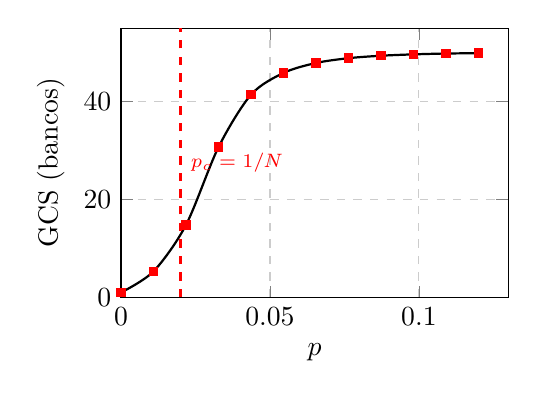
\begin{tikzpicture}
          \begin{axis}[
            ylabel={GCS (bancos)},
            ymin=0, ymax=55,
          ]
          \addplot[red marks] coordinates {
            (0.00001, 1.01)
            (0.01092, 5.33)
            (0.02183, 14.83)
            (0.03273, 30.72)
            (0.04364, 41.42)
            (0.05455, 45.87)
            (0.06546, 47.90)
            (0.07637, 48.88)
            (0.08727, 49.38)
            (0.09818, 49.66)
            (0.10909, 49.83)
            (0.12000, 49.90)
          };
          \addplot[black line] coordinates {
            (0.00001, 1.01)
            (0.01092, 5.33)
            (0.02183, 14.83)
            (0.03273, 30.72)
            (0.04364, 41.42)
            (0.05455, 45.87)
            (0.06546, 47.90)
            (0.07637, 48.88)
            (0.08727, 49.38)
            (0.09818, 49.66)
            (0.10909, 49.83)
            (0.12000, 49.90)
          };
          \draw[red, dashed, thick] (axis cs:0.02,0) -- (axis cs:0.02,55)
            node[pos=0.5, right, font=\scriptsize]{$p_c = 1/N$};
          \end{axis}
        \end{tikzpicture}
      \end{figure}
    \end{column}
    \begin{column}{0.42\textwidth}
      \small
      \textbf{Umbral de percolación} para grafo Erd\H{o}s--R\'enyi:
      \[
        p_c = \frac{1}{N} = \frac{1}{50} = 0.02
      \]
      \vspace{0.3cm}
      \begin{tabular}{rr}
        \toprule
        $p$ & GCS \\
        \midrule
        $10^{-5}$ & 1 \\
        0.011 & 5 \\
        \textbf{0.022} & \textbf{15} \\
        0.033 & 31 \\
        0.044 & 41 \\
        \textbf{0.055} & \textbf{46} \\
        0.065 & 48 \\
        0.087 & 49 \\
        $\geq 0.11$ & 50 \\
        \bottomrule
      \end{tabular}
    \end{column}
  \end{columns}
\end{frame}

\begin{frame}{Componente Gigante: Interpretación}
  \begin{itemize}
    \item En $p = p_c = 0.02$ ocurre la transición de percolación:
    el componente gigante aparece y crece rápidamente.
    \item Para $p \geq 0.055$: GCS $\approx 46$ bancos ($92\%$ del sistema).
    \item Para $p \geq 0.08$: GCS $\approx 50$ ($\sim 100\%$).
    \item \textbf{Conclusión:} la red está saturada de conexiones a partir
    de $p \approx 0.05$, lo que explica la estabilización de todas las
    demás métricas en ese punto.
  \end{itemize}
\end{frame}

% ============================================================
\section{Tasa de Interés}
% ============================================================

\begin{frame}{Tasa de Interés ($ir$)}
  \begin{columns}[T]
    \begin{column}{0.55\textwidth}
      \begin{figure}
        \centering
        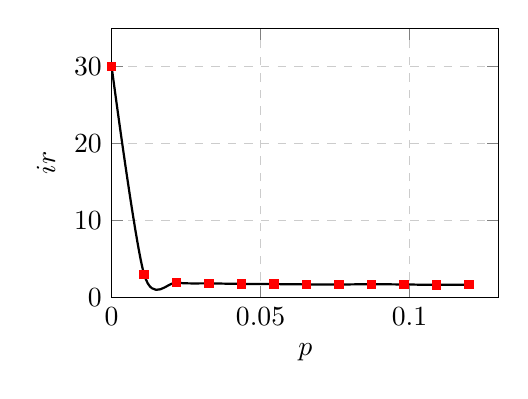
\begin{tikzpicture}
          \begin{axis}[
            ylabel={$ir$},
            ymin=0, ymax=35,
          ]
          \addplot[red marks] coordinates {
            (0.00001, 30.00)
            (0.01092, 2.99)
            (0.02183, 1.92)
            (0.03273, 1.82)
            (0.04364, 1.76)
            (0.05455, 1.73)
            (0.06546, 1.69)
            (0.07637, 1.68)
            (0.08727, 1.71)
            (0.09818, 1.68)
            (0.10909, 1.63)
            (0.12000, 1.66)
          };
          \addplot[black line] coordinates {
            (0.00001, 30.00)
            (0.01092, 2.99)
            (0.02183, 1.92)
            (0.03273, 1.82)
            (0.04364, 1.76)
            (0.05455, 1.73)
            (0.06546, 1.69)
            (0.07637, 1.68)
            (0.08727, 1.71)
            (0.09818, 1.68)
            (0.10909, 1.63)
            (0.12000, 1.66)
          };
          \end{axis}
        \end{tikzpicture}
      \end{figure}
    \end{column}
    \begin{column}{0.42\textwidth}
      \small
      \begin{itemize}
        \item En $p \approx 0$, $ir = 30$ (cap máximo): muy pocos
        prestamistas disponibles $\Rightarrow$ escasez extrema.
        \item Caída brusca: $30 \to 3.0$ con $p = 0.01$.
        \item Estabilización: $ir \approx 1.65$ para $p \geq 0.05$.
        \item \textbf{Mecanismo:} más conexiones $\Rightarrow$ más
        prestamistas $\Rightarrow$ menor riesgo $\Rightarrow$ menor tasa.
      \end{itemize}
      \vspace{0.3cm}
      \small
      \begin{tabular}{rr}
        \toprule
        $p$ & $ir$ \\
        \midrule
        $10^{-5}$ & 30.00 \\
        0.011 & 2.99 \\
        0.022 & 1.92 \\
        0.033 & 1.82 \\
        \textbf{0.055} & \textbf{1.73} \\
        0.087 & 1.71 \\
        0.120 & 1.66 \\
        \bottomrule
      \end{tabular}
    \end{column}
  \end{columns}
\end{frame}

\begin{frame}{Tasa de Interés Ponderada ($ir_w$)}
  \begin{columns}[T]
    \begin{column}{0.55\textwidth}
      \begin{figure}
        \centering
        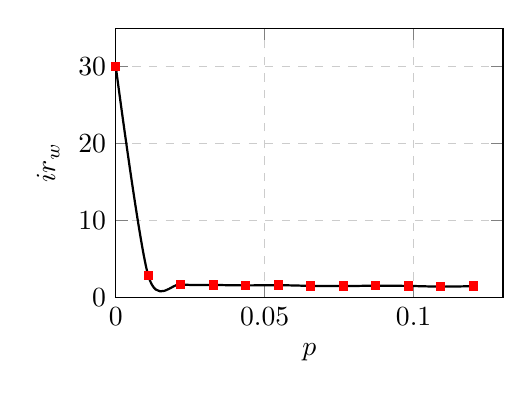
\begin{tikzpicture}
          \begin{axis}[
            ylabel={$ir_w$},
            ymin=0, ymax=35,
          ]
          \addplot[red marks] coordinates {
            (0.00001, 30.00)
            (0.01092, 2.82)
            (0.02183, 1.71)
            (0.03273, 1.62)
            (0.04364, 1.56)
            (0.05455, 1.59)
            (0.06546, 1.50)
            (0.07637, 1.47)
            (0.08727, 1.52)
            (0.09818, 1.49)
            (0.10909, 1.40)
            (0.12000, 1.46)
          };
          \addplot[black line] coordinates {
            (0.00001, 30.00)
            (0.01092, 2.82)
            (0.02183, 1.71)
            (0.03273, 1.62)
            (0.04364, 1.56)
            (0.05455, 1.59)
            (0.06546, 1.50)
            (0.07637, 1.47)
            (0.08727, 1.52)
            (0.09818, 1.49)
            (0.10909, 1.40)
            (0.12000, 1.46)
          };
          \end{axis}
        \end{tikzpicture}
      \end{figure}
    \end{column}
    \begin{column}{0.42\textwidth}
      \small
      \begin{itemize}
        \item $ir_w$ ponderada por volumen de préstamos.
        \item Misma tendencia que $ir$, valores ligeramente menores.
        \item Para $p \geq 0.05$: $ir_w \approx 1.5$.
        \item La ponderación suaviza la media, confirmando
        que los préstamos grandes tienen tasas más bajas.
      \end{itemize}
    \end{column}
  \end{columns}
\end{frame}

% ============================================================
\section{Deuda Incobrable}
% ============================================================

\begin{frame}{Deuda Incobrable ($bad\_debt$)}
  \begin{columns}[T]
    \begin{column}{0.55\textwidth}
      \begin{figure}
        \centering
        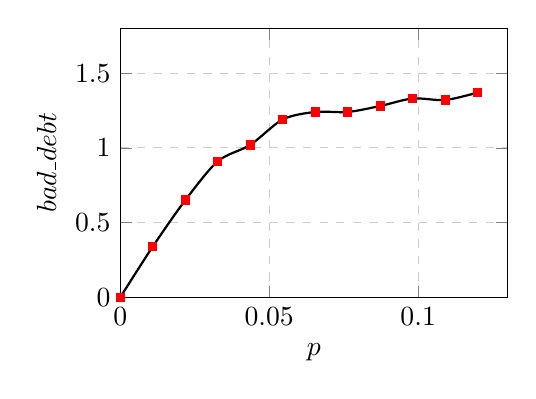
\begin{tikzpicture}
          \begin{axis}[
            ylabel={$bad\_debt$},
            ymin=0, ymax=1.8,
          ]
          \addplot[red marks] coordinates {
            (0.00001, 0.001)
            (0.01092, 0.34)
            (0.02183, 0.65)
            (0.03273, 0.91)
            (0.04364, 1.02)
            (0.05455, 1.19)
            (0.06546, 1.24)
            (0.07637, 1.24)
            (0.08727, 1.28)
            (0.09818, 1.33)
            (0.10909, 1.32)
            (0.12000, 1.37)
          };
          \addplot[black line] coordinates {
            (0.00001, 0.001)
            (0.01092, 0.34)
            (0.02183, 0.65)
            (0.03273, 0.91)
            (0.04364, 1.02)
            (0.05455, 1.19)
            (0.06546, 1.24)
            (0.07637, 1.24)
            (0.08727, 1.28)
            (0.09818, 1.33)
            (0.10909, 1.32)
            (0.12000, 1.37)
          };
          \end{axis}
        \end{tikzpicture}
      \end{figure}
    \end{column}
    \begin{column}{0.42\textwidth}
      \small
      \begin{itemize}
        \item Crecimiento rápido en $p < 0.05$: $0 \to 1.2$.
        \item Crecimiento lento pero continuo para $p > 0.05$:
        $1.2 \to 1.37$.
        \item \textbf{No se satura completamente:}
        la deuda incobrable sigue aumentando suavemente
        porque más conexiones generan más préstamos y
        potencialmente más incumplimientos.
      \end{itemize}
    \end{column}
  \end{columns}
\end{frame}

% ============================================================
\section{Quiebras}
% ============================================================

\begin{frame}{Número de Quiebras}
  \begin{columns}[T]
    \begin{column}{0.55\textwidth}
      \begin{figure}
        \centering
        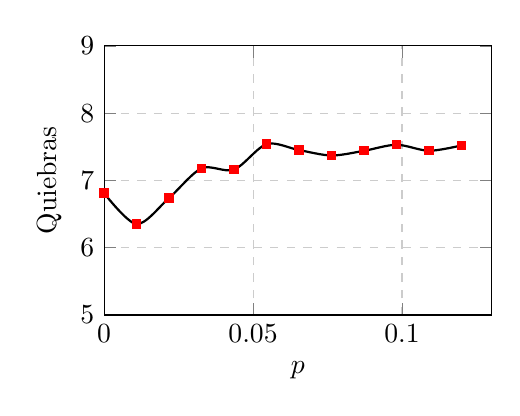
\begin{tikzpicture}
          \begin{axis}[
            ylabel={Quiebras},
            ymin=5, ymax=9,
          ]
          \addplot[red marks] coordinates {
            (0.00001, 6.81)
            (0.01092, 6.35)
            (0.02183, 6.74)
            (0.03273, 7.18)
            (0.04364, 7.16)
            (0.05455, 7.54)
            (0.06546, 7.45)
            (0.07637, 7.37)
            (0.08727, 7.44)
            (0.09818, 7.53)
            (0.10909, 7.44)
            (0.12000, 7.52)
          };
          \addplot[black line] coordinates {
            (0.00001, 6.81)
            (0.01092, 6.35)
            (0.02183, 6.74)
            (0.03273, 7.18)
            (0.04364, 7.16)
            (0.05455, 7.54)
            (0.06546, 7.45)
            (0.07637, 7.37)
            (0.08727, 7.44)
            (0.09818, 7.53)
            (0.10909, 7.44)
            (0.12000, 7.52)
          };
          \end{axis}
        \end{tikzpicture}
      \end{figure}
    \end{column}
    \begin{column}{0.42\textwidth}
      \small
      \begin{itemize}
        \item Quiebras estables entre $6.8$ y $7.5$.
        \item Leve incremento al inicio ($p < 0.05$).
        \item Para $p > 0.05$: se estabiliza en $\sim 7.5$.
        \item \textbf{Interpretación:} más conexiones facilitan
        la propagación de quiebras (contagio), pero el
        número de quiebras está limitado por la estructura
        del modelo.
      \end{itemize}
    \end{column}
  \end{columns}
\end{frame}

% ============================================================
\section{Préstamos}
% ============================================================

\begin{frame}{Número de Préstamos Activos}
  \begin{columns}[T]
    \begin{column}{0.55\textwidth}
      \begin{figure}
        \centering
        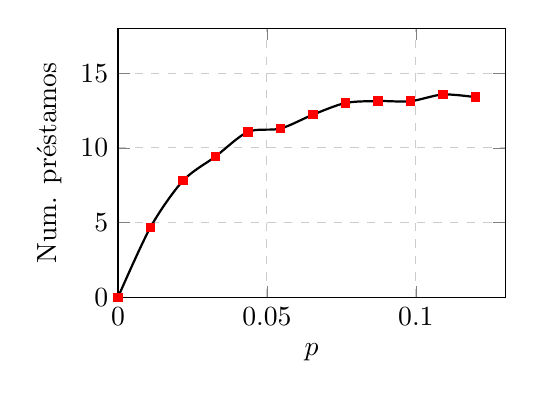
\begin{tikzpicture}
          \begin{axis}[
            ylabel={Num. préstamos},
            ymin=0, ymax=18,
          ]
          \addplot[red marks] coordinates {
            (0.00001, 0.004)
            (0.01092, 4.69)
            (0.02183, 7.80)
            (0.03273, 9.42)
            (0.04364, 11.07)
            (0.05455, 11.29)
            (0.06546, 12.22)
            (0.07637, 13.00)
            (0.08727, 13.13)
            (0.09818, 13.12)
            (0.10909, 13.57)
            (0.12000, 13.39)
          };
          \addplot[black line] coordinates {
            (0.00001, 0.004)
            (0.01092, 4.69)
            (0.02183, 7.80)
            (0.03273, 9.42)
            (0.04364, 11.07)
            (0.05455, 11.29)
            (0.06546, 12.22)
            (0.07637, 13.00)
            (0.08727, 13.13)
            (0.09818, 13.12)
            (0.10909, 13.57)
            (0.12000, 13.39)
          };
          \end{axis}
        \end{tikzpicture}
      \end{figure}
    \end{column}
    \begin{column}{0.42\textwidth}
      \small
      \begin{itemize}
        \item Crecimiento rápido en $p < 0.05$: $0 \to 11$.
        \item Meseta parcial en $p > 0.05$: $\sim 13$ préstamos.
        \item Solo $\sim 26\%$ de los bancos necesitan préstamos
        simultáneamente ($13/50$).
        \item \textbf{Saturación:} la demanda de préstamos está
        limitada por la estructura del modelo, no por la
        oferta de crédito.
      \end{itemize}
    \end{column}
  \end{columns}
\end{frame}

% ============================================================
\section{Patrimonio}
% ============================================================

\begin{frame}{Patrimonio Promedio ($equity$)}
  \begin{columns}[T]
    \begin{column}{0.55\textwidth}
      \begin{figure}
        \centering
        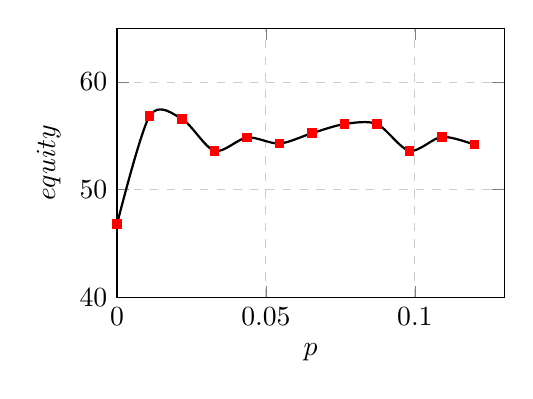
\begin{tikzpicture}
          \begin{axis}[
            ylabel={$equity$},
            ymin=40, ymax=65,
          ]
          \addplot[red marks] coordinates {
            (0.00001, 46.80)
            (0.01092, 56.83)
            (0.02183, 56.57)
            (0.03273, 53.61)
            (0.04364, 54.85)
            (0.05455, 54.29)
            (0.06546, 55.25)
            (0.07637, 56.10)
            (0.08727, 56.10)
            (0.09818, 53.61)
            (0.10909, 54.91)
            (0.12000, 54.18)
          };
          \addplot[black line] coordinates {
            (0.00001, 46.80)
            (0.01092, 56.83)
            (0.02183, 56.57)
            (0.03273, 53.61)
            (0.04364, 54.85)
            (0.05455, 54.29)
            (0.06546, 55.25)
            (0.07637, 56.10)
            (0.08727, 56.10)
            (0.09818, 53.61)
            (0.10909, 54.91)
            (0.12000, 54.18)
          };
          \end{axis}
        \end{tikzpicture}
      \end{figure}
    \end{column}
    \begin{column}{0.42\textwidth}
      \small
      \begin{itemize}
        \item Salto inicial: $46.8 \to 56.8$ con $p = 0.01$
        (más préstamos $\Rightarrow$ más ingresos por intereses).
        \item Meseta ruidosa: $equity \approx 54$--$56$ para
        $p > 0.01$.
        \item El patrimonio no mejora con más conexiones
        más allá de $p \approx 0.01$.
      \end{itemize}
    \end{column}
  \end{columns}
\end{frame}

% ============================================================
\section{Leverage y Liquidez}
% ============================================================

\begin{frame}{Leverage y Liquidez}
  \begin{columns}[T]
    \begin{column}{0.48\textwidth}
      \small\textbf{Leverage}
      \begin{figure}
        \centering
        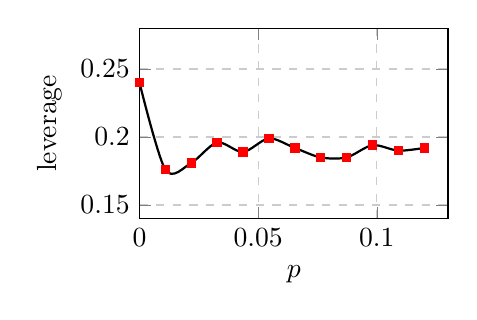
\begin{tikzpicture}
          \begin{axis}[
            width=5.5cm, height=4cm,
            ylabel={leverage},
            xmin=0, xmax=0.13, ymin=0.14, ymax=0.28,
            grid=major, grid style={dashed,gray!40},
            mark size=1.5pt,
            xlabel={$p$},
            xticklabel style={/pgf/number format/fixed, /pgf/number format/precision=2},
          ]
          \addplot[red marks] coordinates {
            (0.00001, 0.240)
            (0.01092, 0.176)
            (0.02183, 0.181)
            (0.03273, 0.196)
            (0.04364, 0.189)
            (0.05455, 0.199)
            (0.06546, 0.192)
            (0.07637, 0.185)
            (0.08727, 0.185)
            (0.09818, 0.194)
            (0.10909, 0.190)
            (0.12000, 0.192)
          };
          \addplot[black line] coordinates {
            (0.00001, 0.240)
            (0.01092, 0.176)
            (0.02183, 0.181)
            (0.03273, 0.196)
            (0.04364, 0.189)
            (0.05455, 0.199)
            (0.06546, 0.192)
            (0.07637, 0.185)
            (0.08727, 0.185)
            (0.09818, 0.194)
            (0.10909, 0.190)
            (0.12000, 0.192)
          };
          \end{axis}
        \end{tikzpicture}
      \end{figure}
    \end{column}
    \begin{column}{0.48\textwidth}
      \small\textbf{Liquidez}
      \begin{figure}
        \centering
        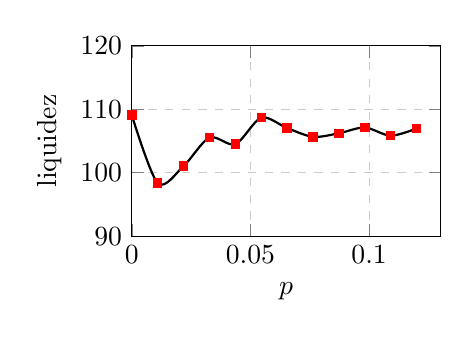
\begin{tikzpicture}
          \begin{axis}[
            width=5.5cm, height=4cm,
            ylabel={liquidez},
            xmin=0, xmax=0.13, ymin=90, ymax=120,
            grid=major, grid style={dashed,gray!40},
            mark size=1.5pt,
            scaled x ticks=false,
            xlabel={$p$},
          ]
          \addplot[red marks] coordinates {
            (0.00001, 109.08)
            (0.01092, 98.37)
            (0.02183, 101.06)
            (0.03273, 105.54)
            (0.04364, 104.50)
            (0.05455, 108.68)
            (0.06546, 107.04)
            (0.07637, 105.66)
            (0.08727, 106.22)
            (0.09818, 107.13)
            (0.10909, 105.84)
            (0.12000, 106.97)
          };
          \addplot[black line] coordinates {
            (0.00001, 109.08)
            (0.01092, 98.37)
            (0.02183, 101.06)
            (0.03273, 105.54)
            (0.04364, 104.50)
            (0.05455, 108.68)
            (0.06546, 107.04)
            (0.07637, 105.66)
            (0.08727, 106.22)
            (0.09818, 107.13)
            (0.10909, 105.84)
            (0.12000, 106.97)
          };
          \end{axis}
        \end{tikzpicture}
      \end{figure}
    \end{column}
  \end{columns}
  \vspace{0.3cm}
  \small
  Ambas métricas son \textbf{estables} para todo $p > 0.01$.
  El leverage se mantiene en $\sim 0.19$ y la liquidez en $\sim 106$.
\end{frame}

% ============================================================
\section{Medidas de Riesgo Extremo}
% ============================================================

\begin{frame}{Estimador de Hill y Curtosis}
  \begin{columns}[T]
    \begin{column}{0.48\textwidth}
      \small\textbf{Hill exponent (equity losses)}
      \begin{figure}
        \centering
        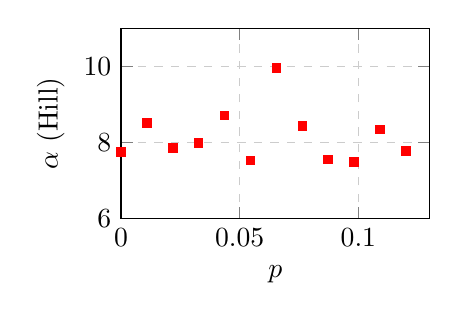
\begin{tikzpicture}
          \begin{axis}[
            width=5.5cm, height=4cm,
            ylabel={$\alpha$ (Hill)},
            xmin=0, xmax=0.13, ymin=6, ymax=11,
            grid=major, grid style={dashed,gray!40},
            mark size=1.5pt,
            scaled x ticks=false,
            xlabel={$p$},
          ]
          \addplot[red marks] coordinates {
            (0.00001, 7.75)
            (0.01092, 8.51)
            (0.02183, 7.85)
            (0.03273, 7.99)
            (0.04364, 8.71)
            (0.05455, 7.53)
            (0.06546, 9.96)
            (0.07637, 8.43)
            (0.08727, 7.56)
            (0.09818, 7.49)
            (0.10909, 8.34)
            (0.12000, 7.78)
          };
          \end{axis}
        \end{tikzpicture}
      \end{figure}
    \end{column}
    \begin{column}{0.48\textwidth}
      \small\textbf{Kurtosis del patrimonio}
      \begin{figure}
        \centering
        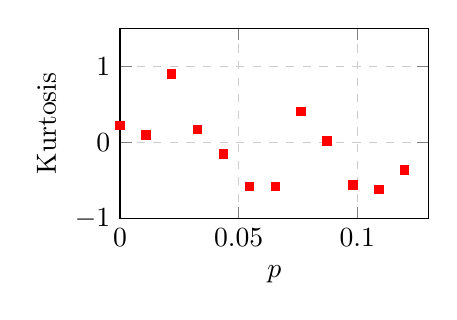
\begin{tikzpicture}
          \begin{axis}[
            width=5.5cm, height=4cm,
            ylabel={Kurtosis},
            xmin=0, xmax=0.13, ymin=-1, ymax=1.5,
            grid=major, grid style={dashed,gray!40},
            mark size=1.5pt,
            scaled x ticks=false,
            xlabel={$p$},
          ]
          \addplot[red marks] coordinates {
            (0.00001, 0.22)
            (0.01092, 0.10)
            (0.02183, 0.90)
            (0.03273, 0.17)
            (0.04364, -0.15)
            (0.05455, -0.58)
            (0.06546, -0.58)
            (0.07637, 0.41)
            (0.08727, 0.02)
            (0.09818, -0.56)
            (0.10909, -0.62)
            (0.12000, -0.36)
          };
          \end{axis}
        \end{tikzpicture}
      \end{figure}
    \end{column}
  \end{columns}
  \vspace{0.3cm}
  \small
  \begin{itemize}
    \item Hill $\alpha \approx 7$--$9$: colas más pesadas que lo esperado
    para datos financieros ($\alpha \in [2,4]$), pero estable con $p$.
    \item Kurtosis ruidosa pero sin tendencia clara: la distribución
    del patrimonio no cambia estructuralmente con $p$.
  \end{itemize}
\end{frame}

% ============================================================
\section{Conclusiones}
% ============================================================

\begin{frame}{Conclusiones Principales}
  \begin{enumerate}
    \item \textbf{Zona de transición} ($p = 0.01$--$0.05$):
    todas las métricas cambian drásticamente en este rango.
    \item \textbf{Saturación de la red:} el componente gigante
    alcanza el $92\%$ de los bancos en $p \approx 0.05$.
    Agregar conexiones más allá de este punto no
    modifica el comportamiento del sistema.
    \item \textbf{Tasa de interés:} cae de 30 (escasez) a $\sim 1.65$
    (equilibrio) con un costo de oportunidad mínimo.
    \item \textbf{Deuda incobrable:} crece rápidamente con $p$ pero
    se estabiliza; nunca llega a cero porque más conexiones
    generan más préstamos con riesgo.
    \item \textbf{Quiebras:} estables en $\sim 7$--$7.5$ bancos;
    el contagio está limitado por la estructura del modelo.
    \item \textbf{Préstamos:} solo el $26\%$ de los bancos necesita
    financiamiento simultáneamente; la demanda, no la oferta,
    es el factor limitante.
  \end{enumerate}
\end{frame}

\begin{frame}{Resultados Clave}
  \begin{center}
    \small
    \begin{tabular}{lcc}
      \toprule
      \textbf{Métrica} & \textbf{Transición} & \textbf{Meseta} \\
      \midrule
      GCS (bancos) & 1 $\to$ 46 & 46--50 \\
      $ir$ & 30 $\to$ 1.73 & $\sim 1.65$ \\
      $ir_w$ & 30 $\to$ 1.59 & $\sim 1.45$ \\
      $bad\_debt$ & 0 $\to$ 1.2 & 1.2--1.4 \\
      Quiebras & 6.8 $\to$ 7.5 & $\sim 7.5$ \\
      Num. préstamos & 0 $\to$ 11 & 11--14 \\
      $equity$ & 46.8 $\to$ 56.8 & 54--56 \\
      \bottomrule
    \end{tabular}
  \end{center}
  \vspace{0.5cm}
  \small
  \textbf{Punto de saturación:} $p \approx 0.05$, donde el $92\%$
  de los bancos están conectados y todas las métricas se estabilizan.
\end{frame}

\begin{frame}
  \begin{center}
    \Large \textbf{Fin de la presentación}
  \end{center}
\end{frame}

\end{document}
